% doc: noticies molt i molt/Revista 1r de primaria.doc
\begin{news}
{3} %columnes
{Notícies molt i molt importants a 1r de Primària}
{Lectoescriptura}
{Primària}
{301} %pagesof


L'aprenentatge de la lectoescriptura és, a primer de primària, un dels aspectes més engrescadors i motivadors per aquest curs, però a la vegada és un procés lent, feixuc i que necessita el seu temps. Qualsevol excusa és bona perquè els nens i nenes d'aquestes edats escriguin. Fer la llista de la compra, notes recordatòries, missatges secrets...Són ,recursos que ajudaran perquè d'una manera espontània i fora de l'àmbit escolar s'engresquin en aquesta difícil tasca que ja van iniciar a Parvulari.

Com cada any, a primer de primària, només començar el curs escolar, es proposa als nens i nenes que si tenen alguna notícia, de caire personal a explicar a la resta de la classe, la facin per escrit i a casa. Durant el  dia es dedica una estona, a llegir-la i a mostrar-la als companys. 

Els primers dies, tímidament, alguns nens i nenes en comencen a escriure i a mida que passen les setmanes, els altres es van animant i cada vegada són més els que hi dediquen més estones.

L'estona de lectura de les notícies és una estona de molta tranquil.litat, tothom escolta. El/la nen/a que llegeix la seva notícia és el protagonista i és el seu moment. Li fem preguntes, com ha succeït el fet, ... Després, la mostra i l'enganxa al mural de notícies.

Heus aquí una mostra de les que han començat a arribar aquest 1r trimestre. Algunes són divertides, d'altres expliquen experiències de cap de setmana, d'altres incidents de caire quotidià, ... La temàtica és molt extensa i diversa.


\end{news}

\begin{news}
{2} %columnes
{}
{}
{}
{01} %pagesof


\noindent\fbox{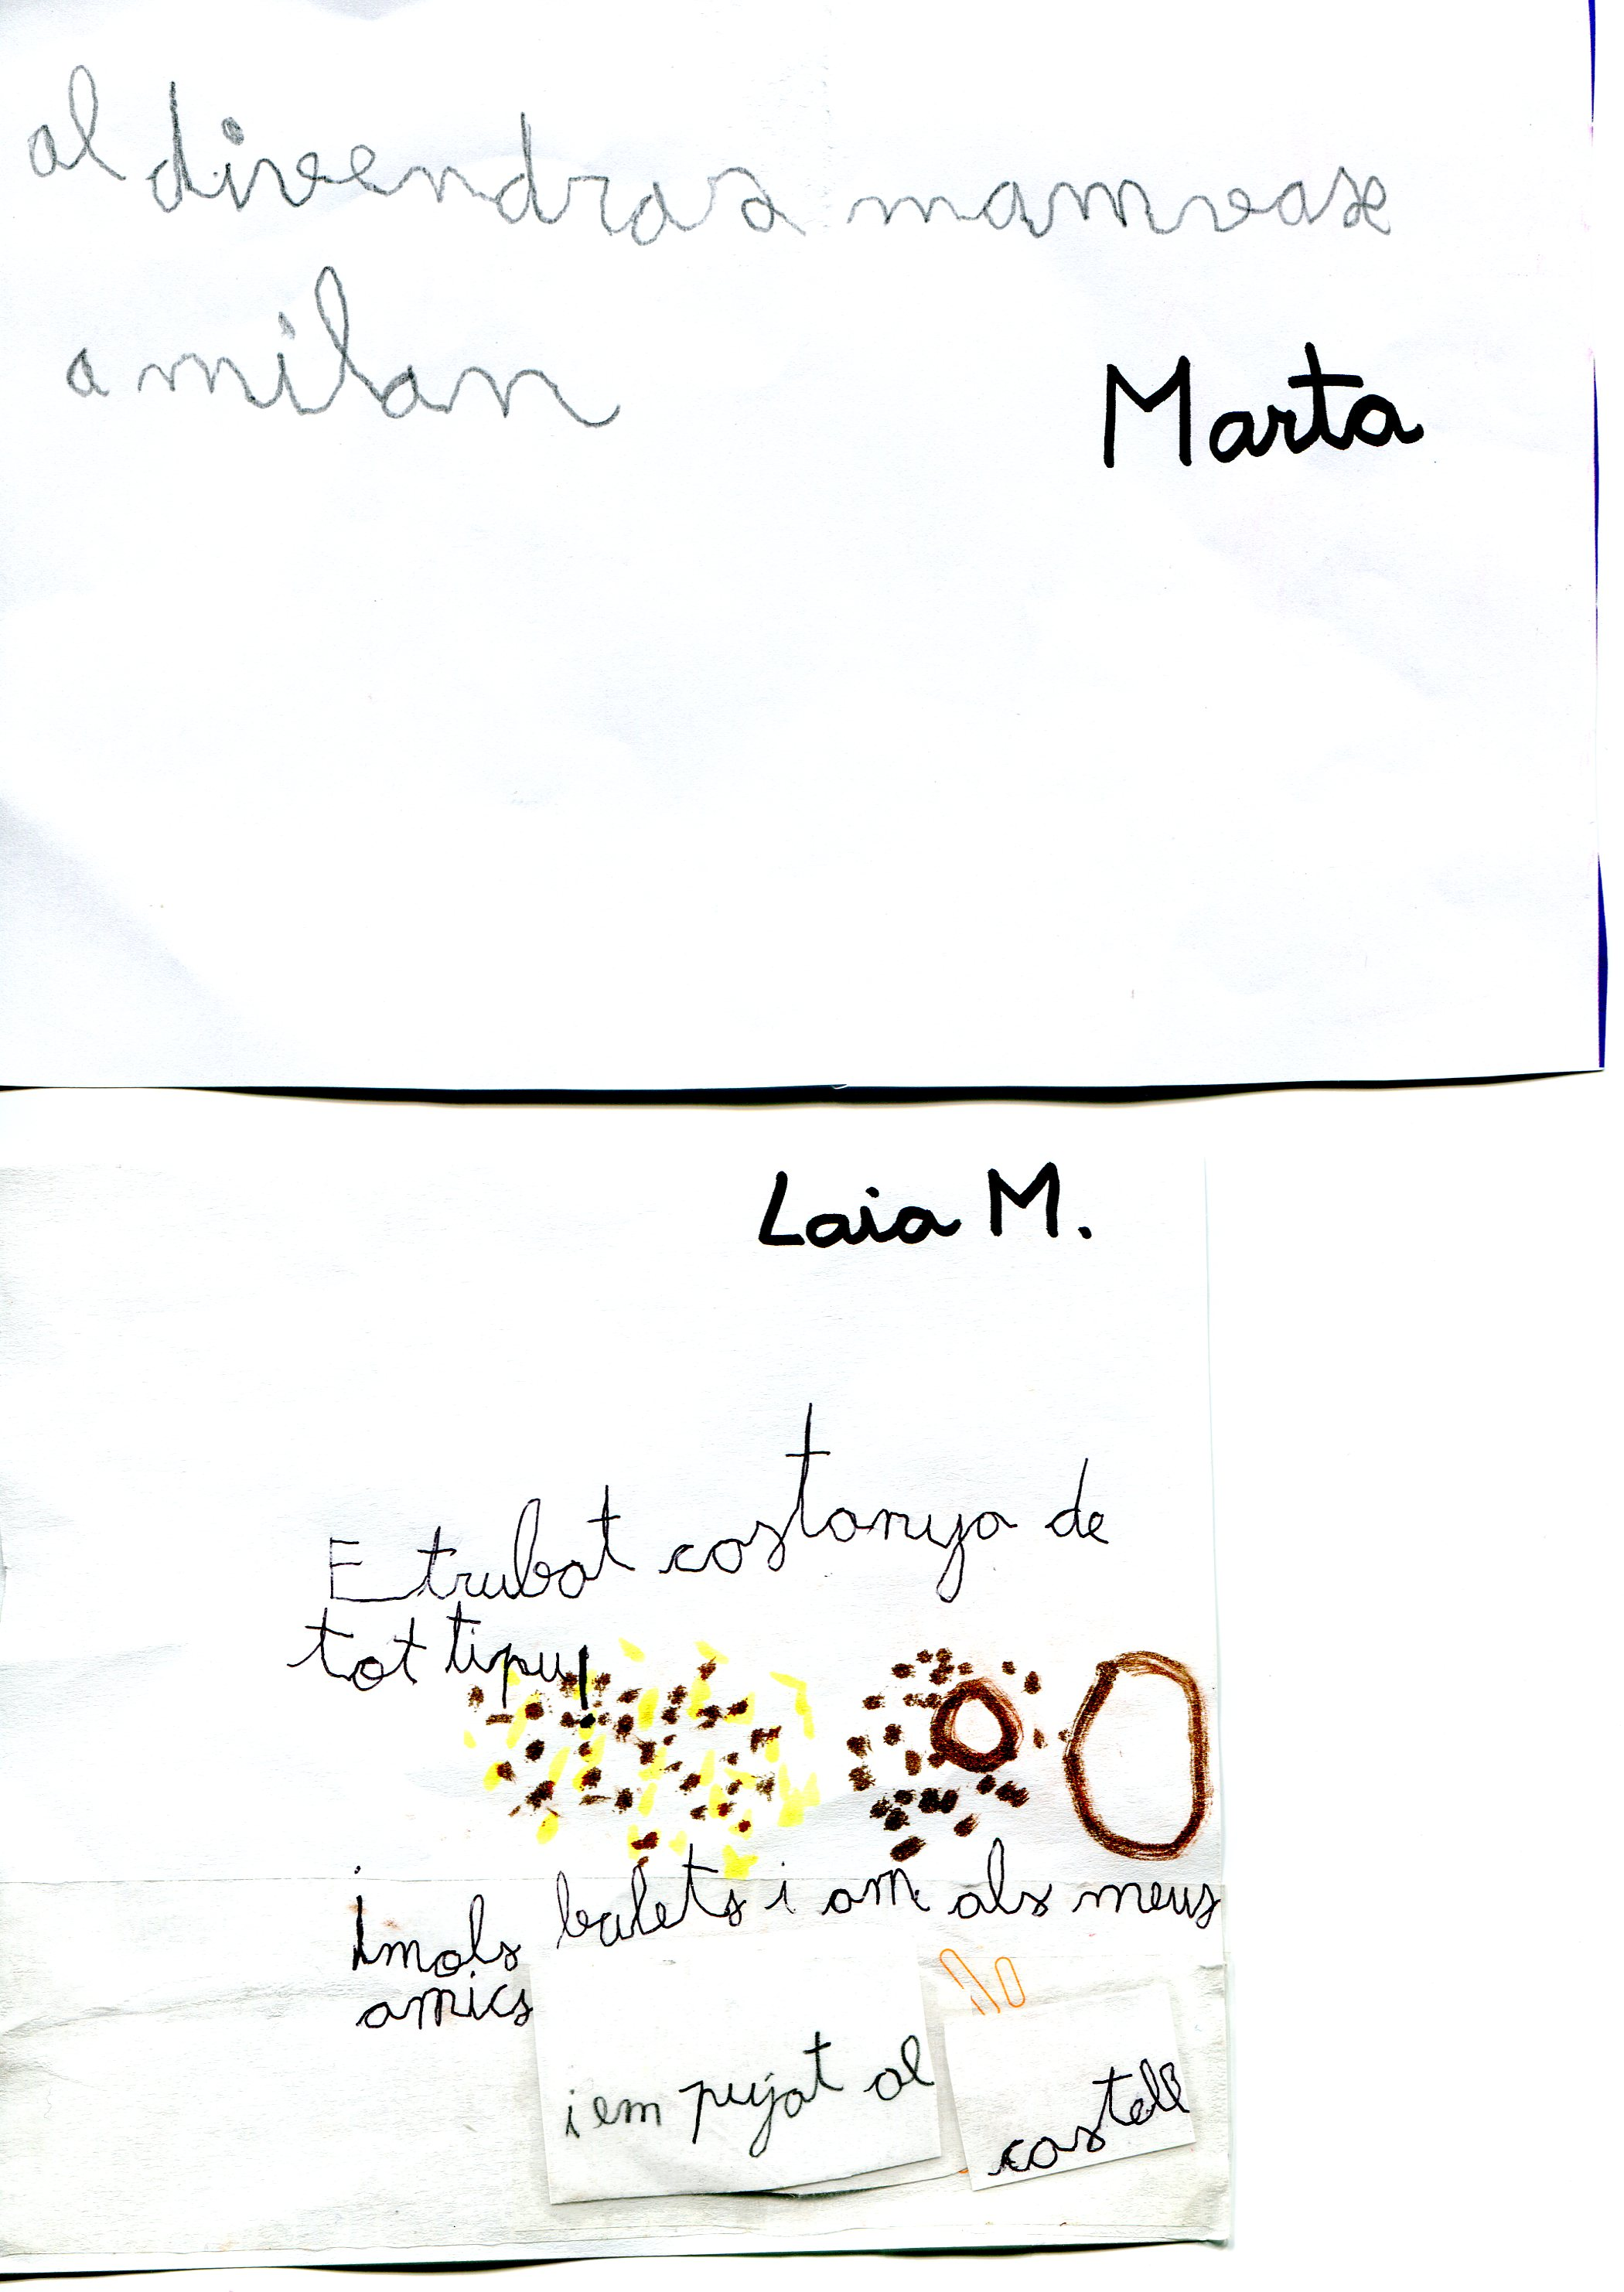
\includegraphics[width=8.4cm,keepaspectratio]{primaria/img/img007.jpg}}

\noindent\fbox{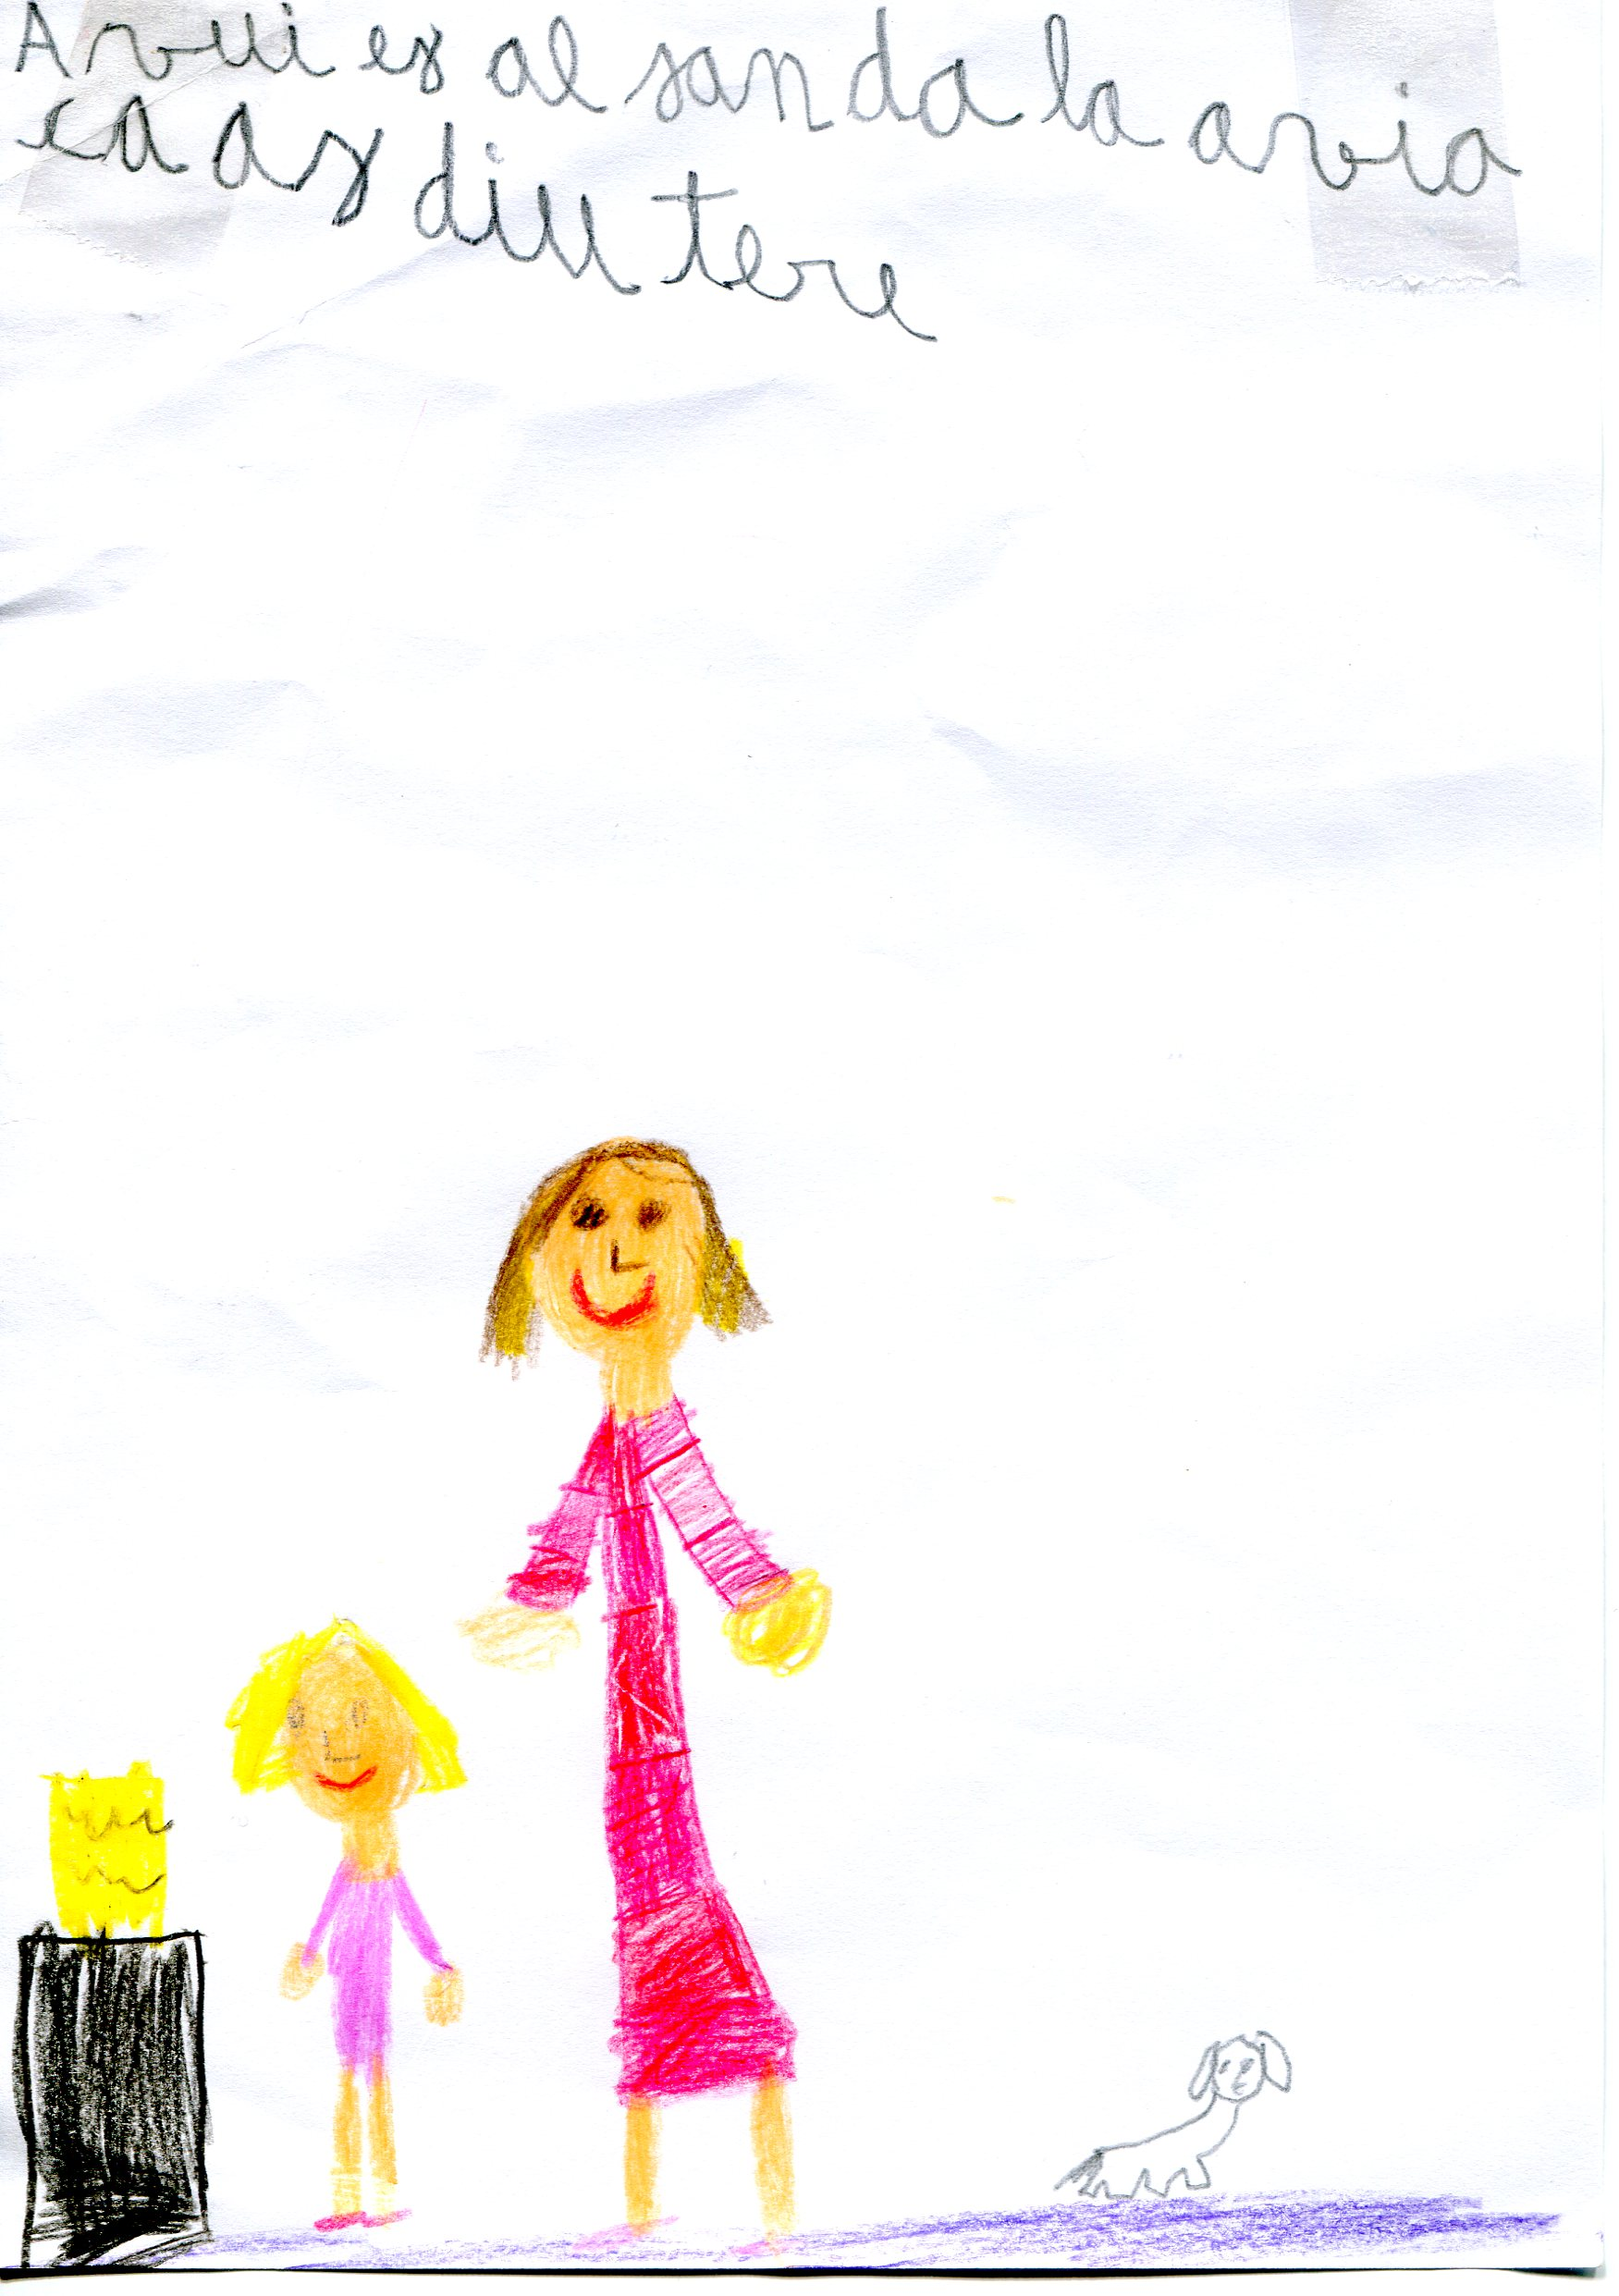
\includegraphics[width=8.4cm,keepaspectratio]{primaria/img/img015.jpg}}

\noindent\fbox{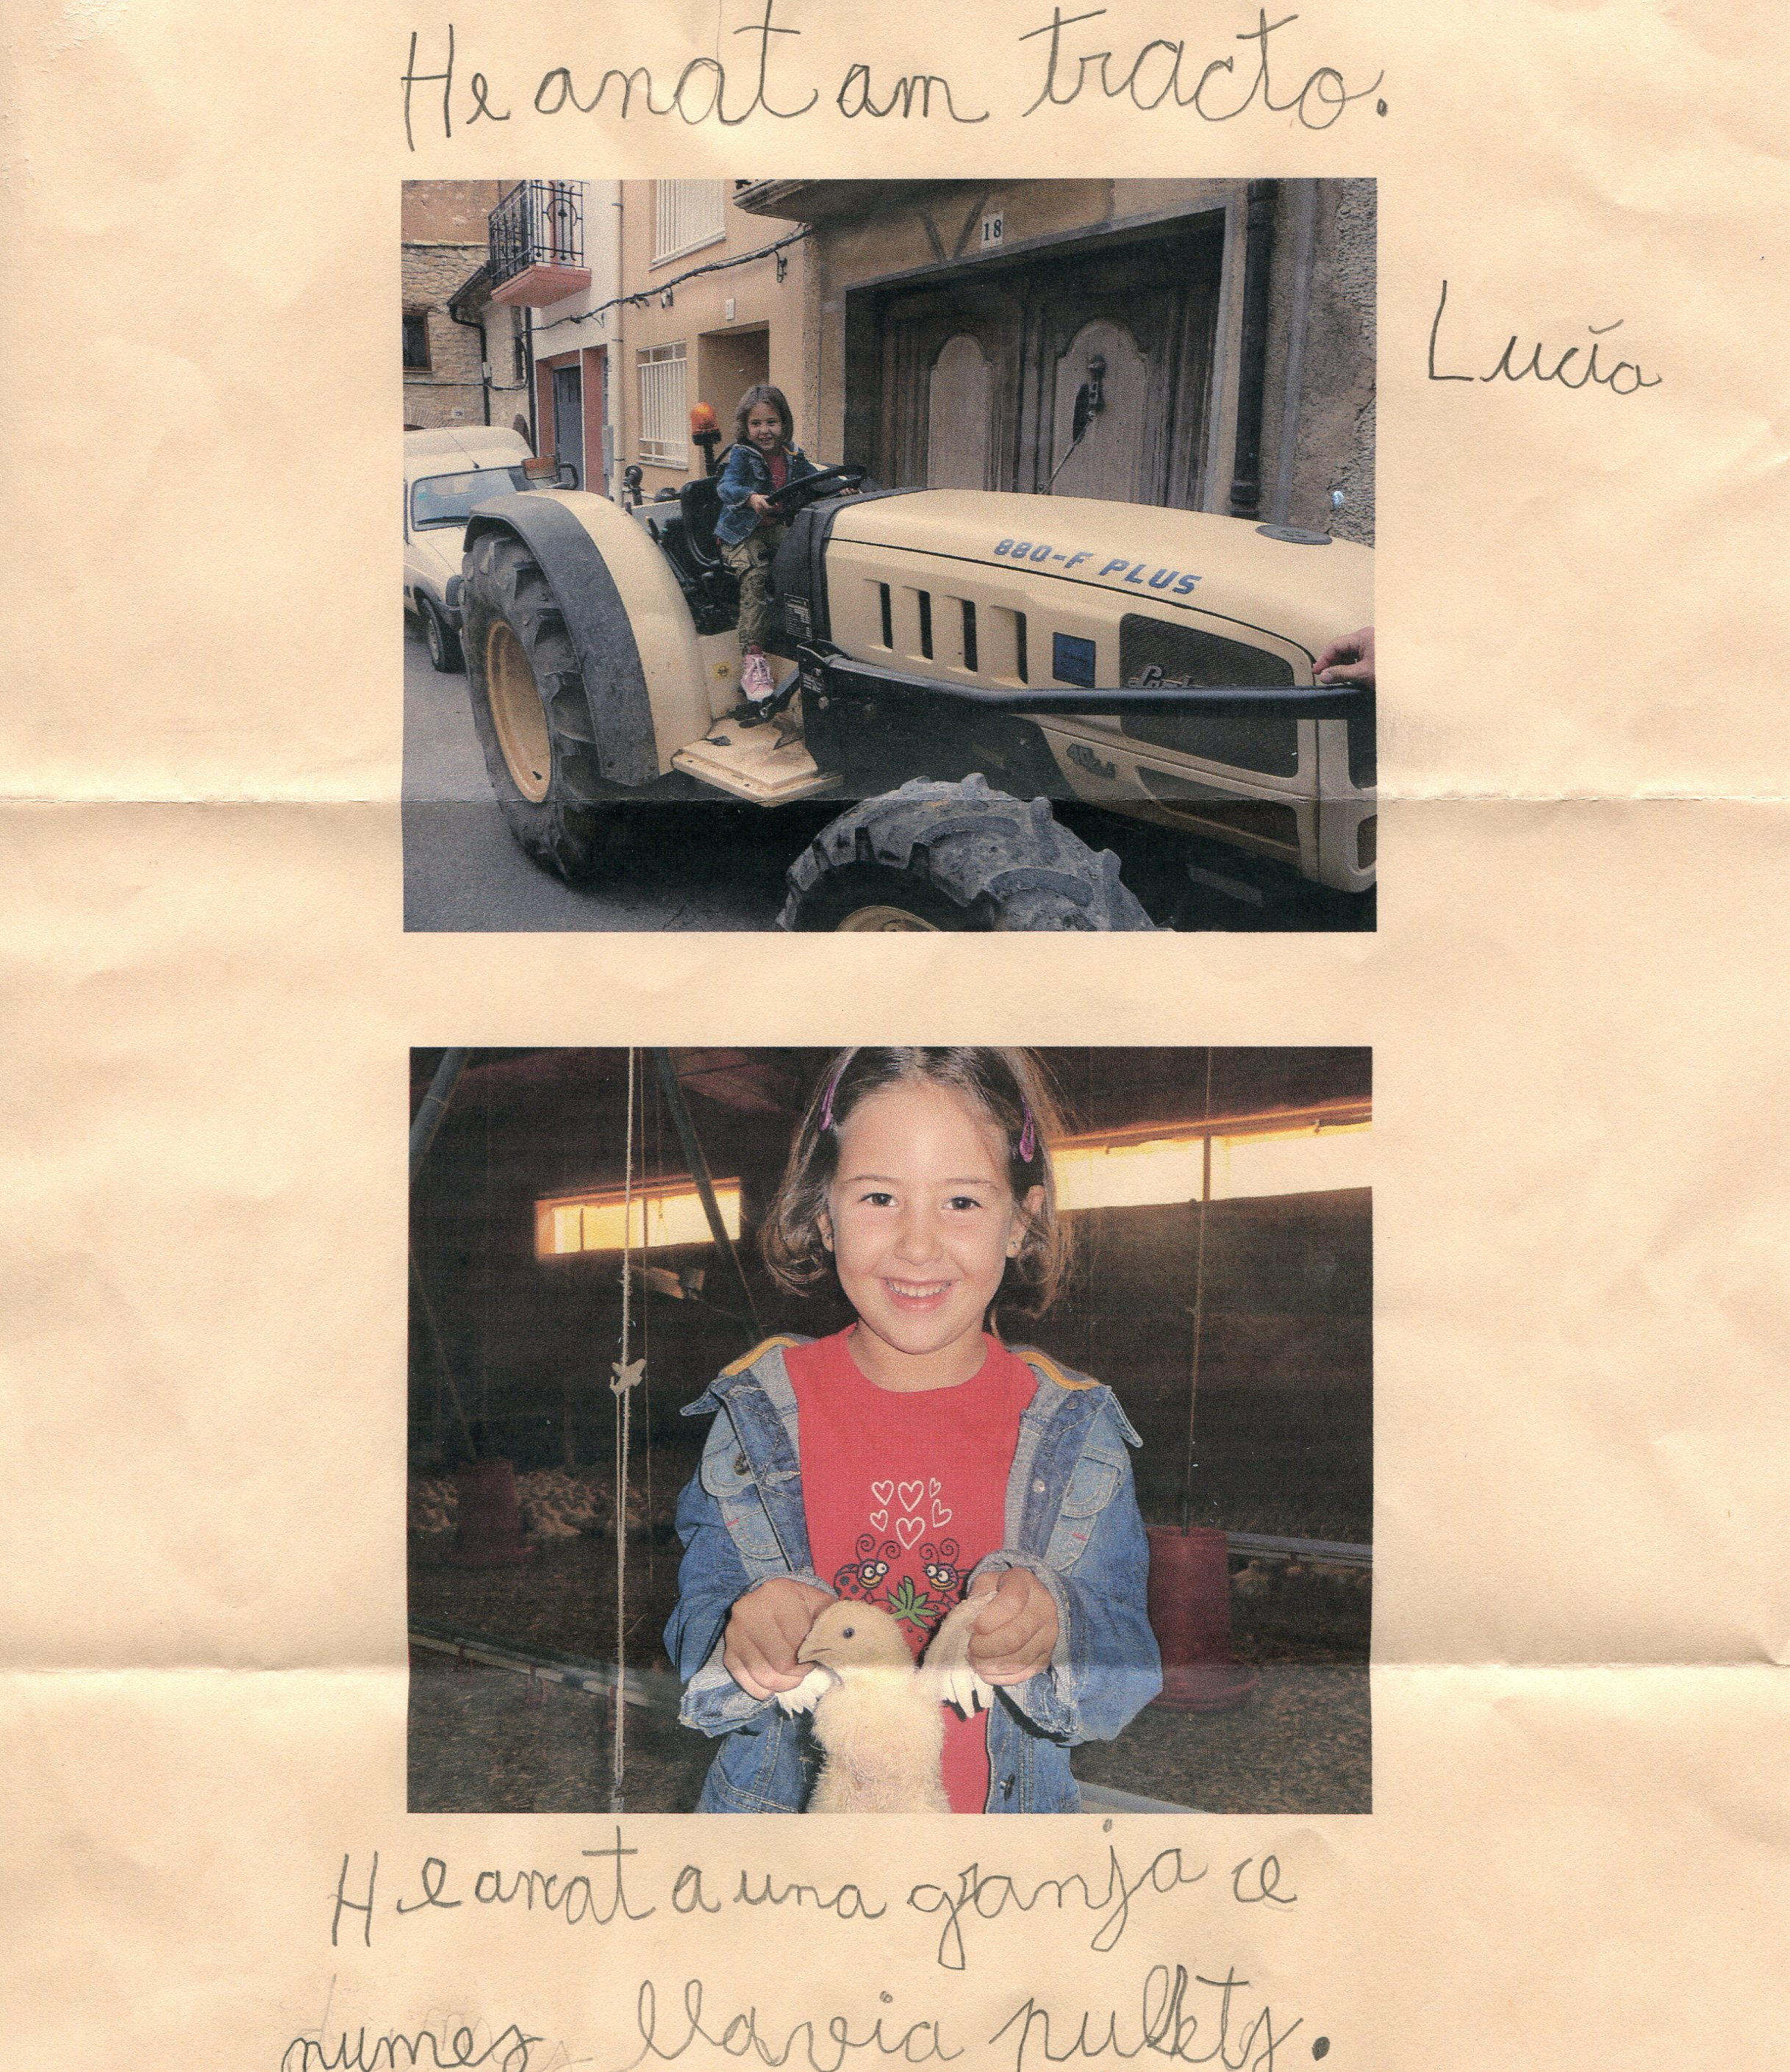
\includegraphics[width=8.4cm,keepaspectratio]{primaria/img/img008.jpg}}

\noindent\fbox{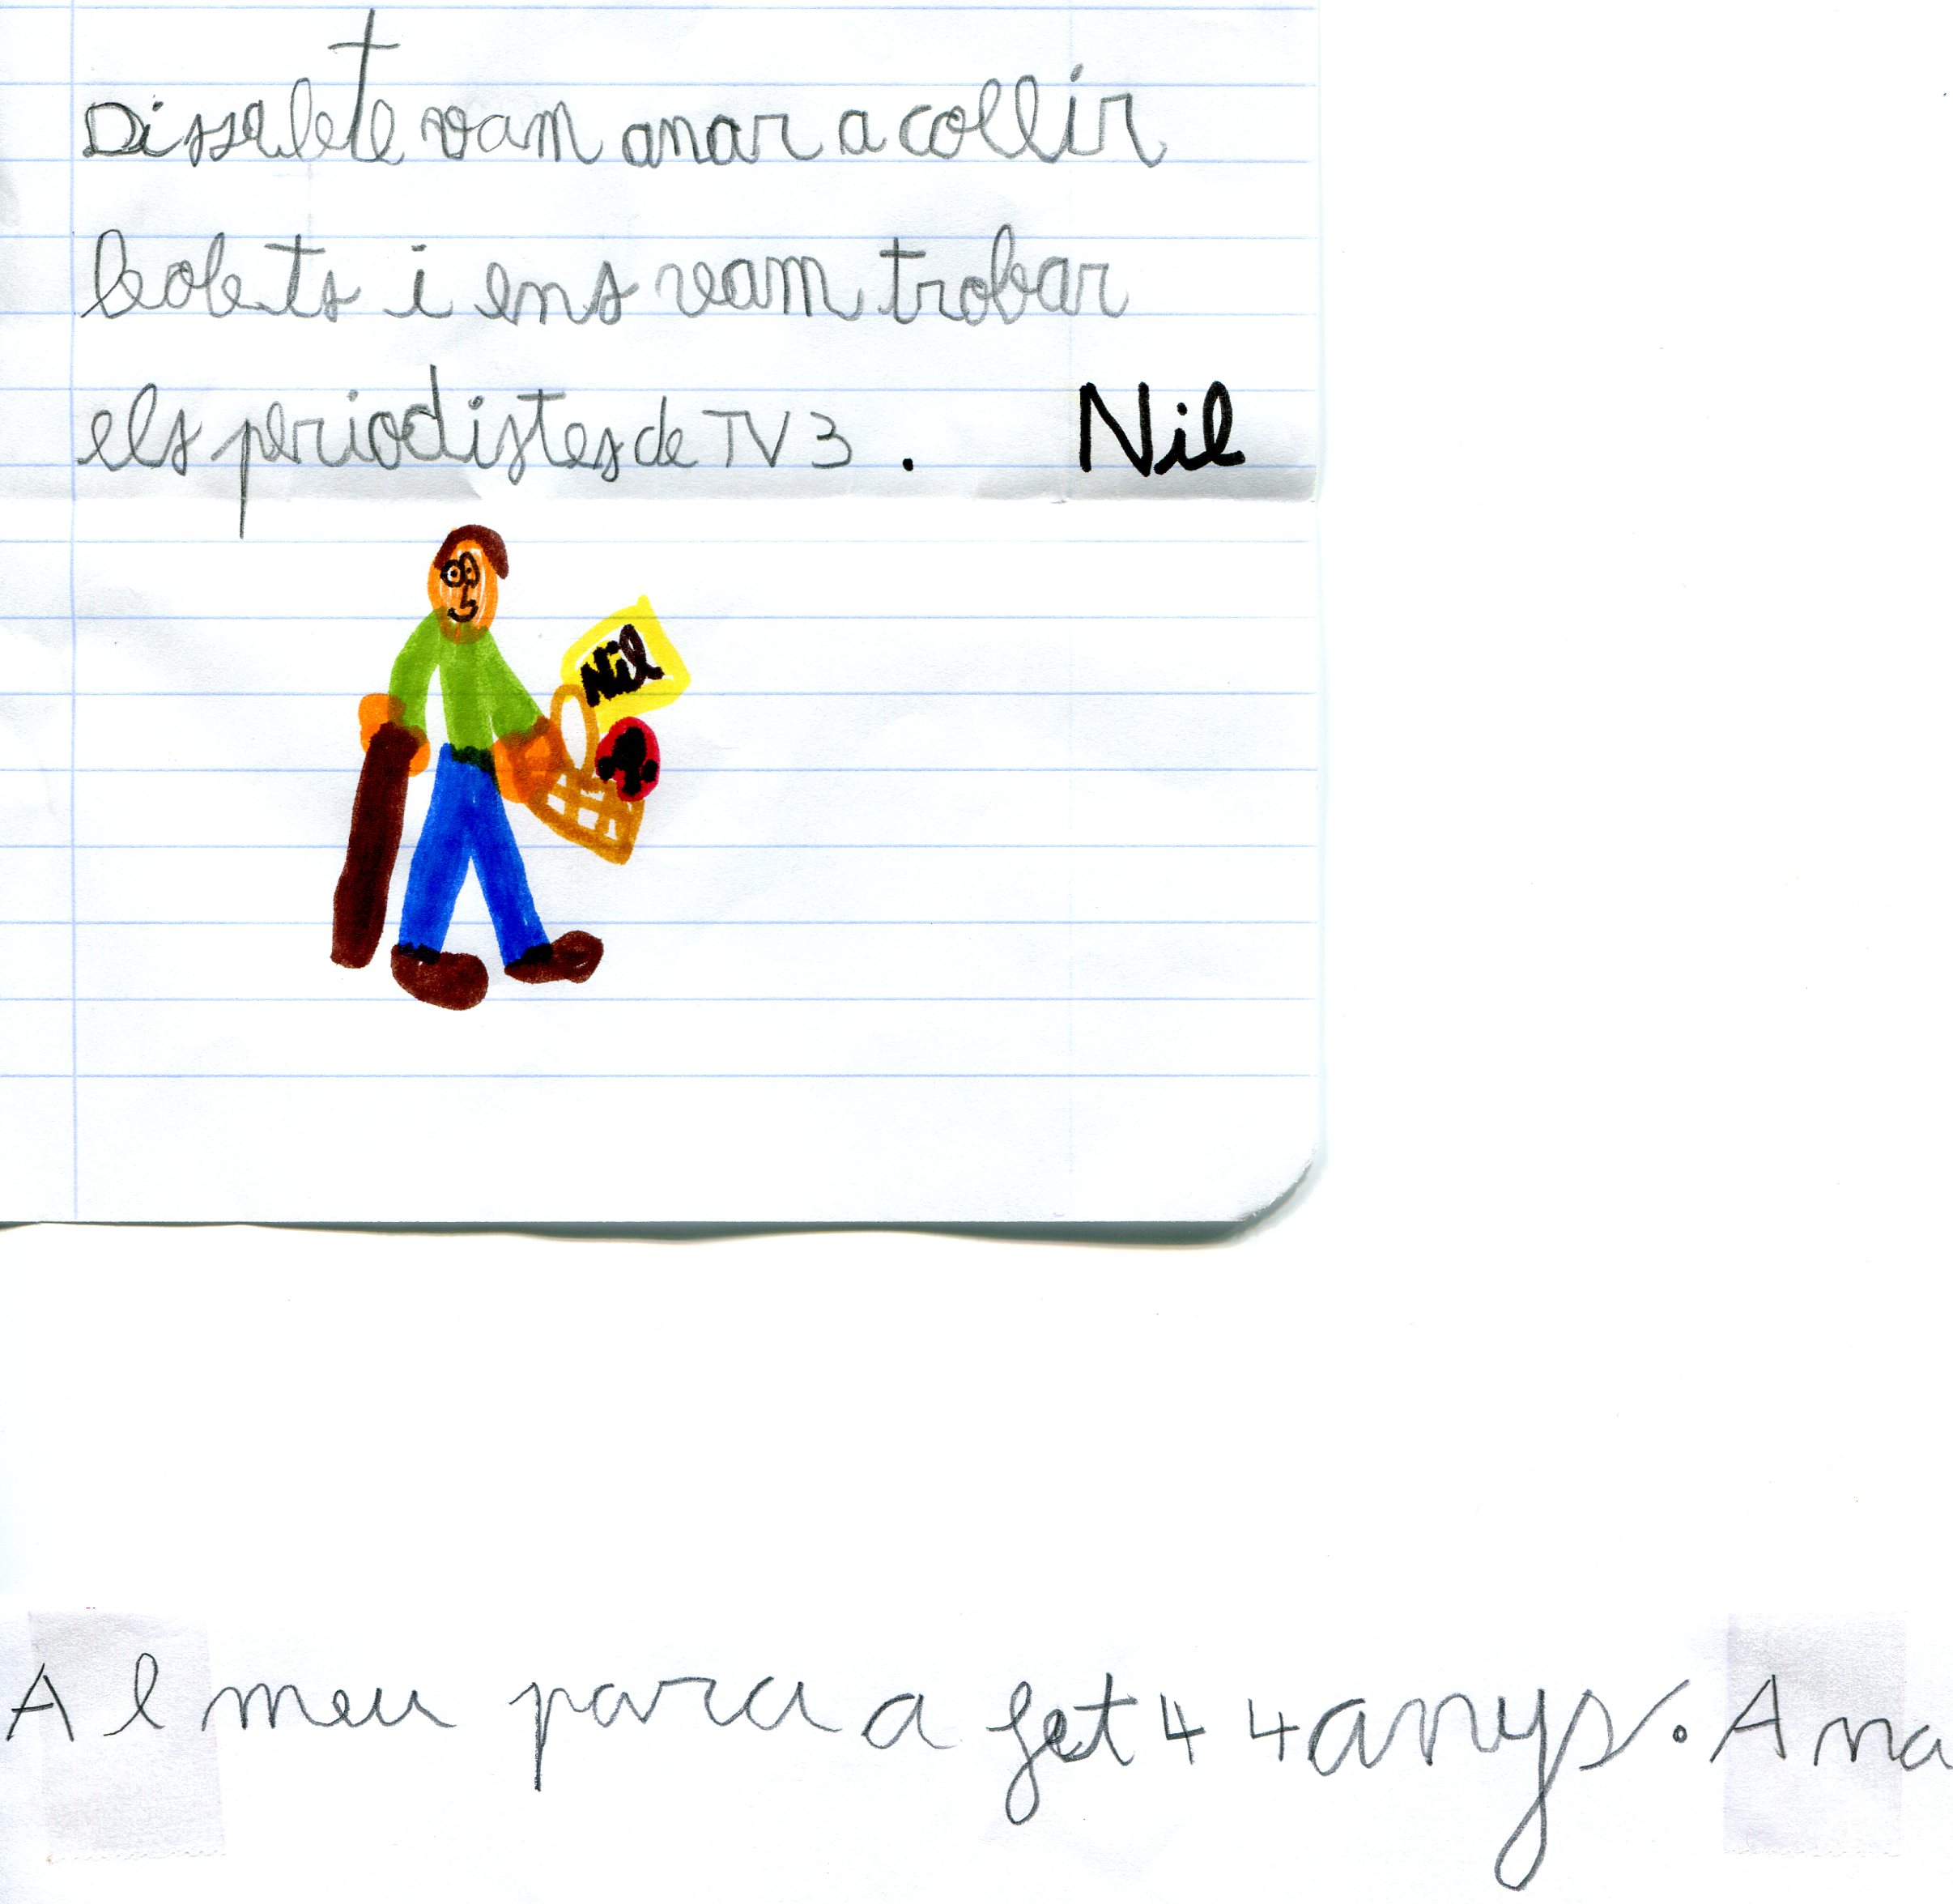
\includegraphics[width=8.4cm,keepaspectratio]{primaria/img/img009.jpg}}

\noindent\fbox{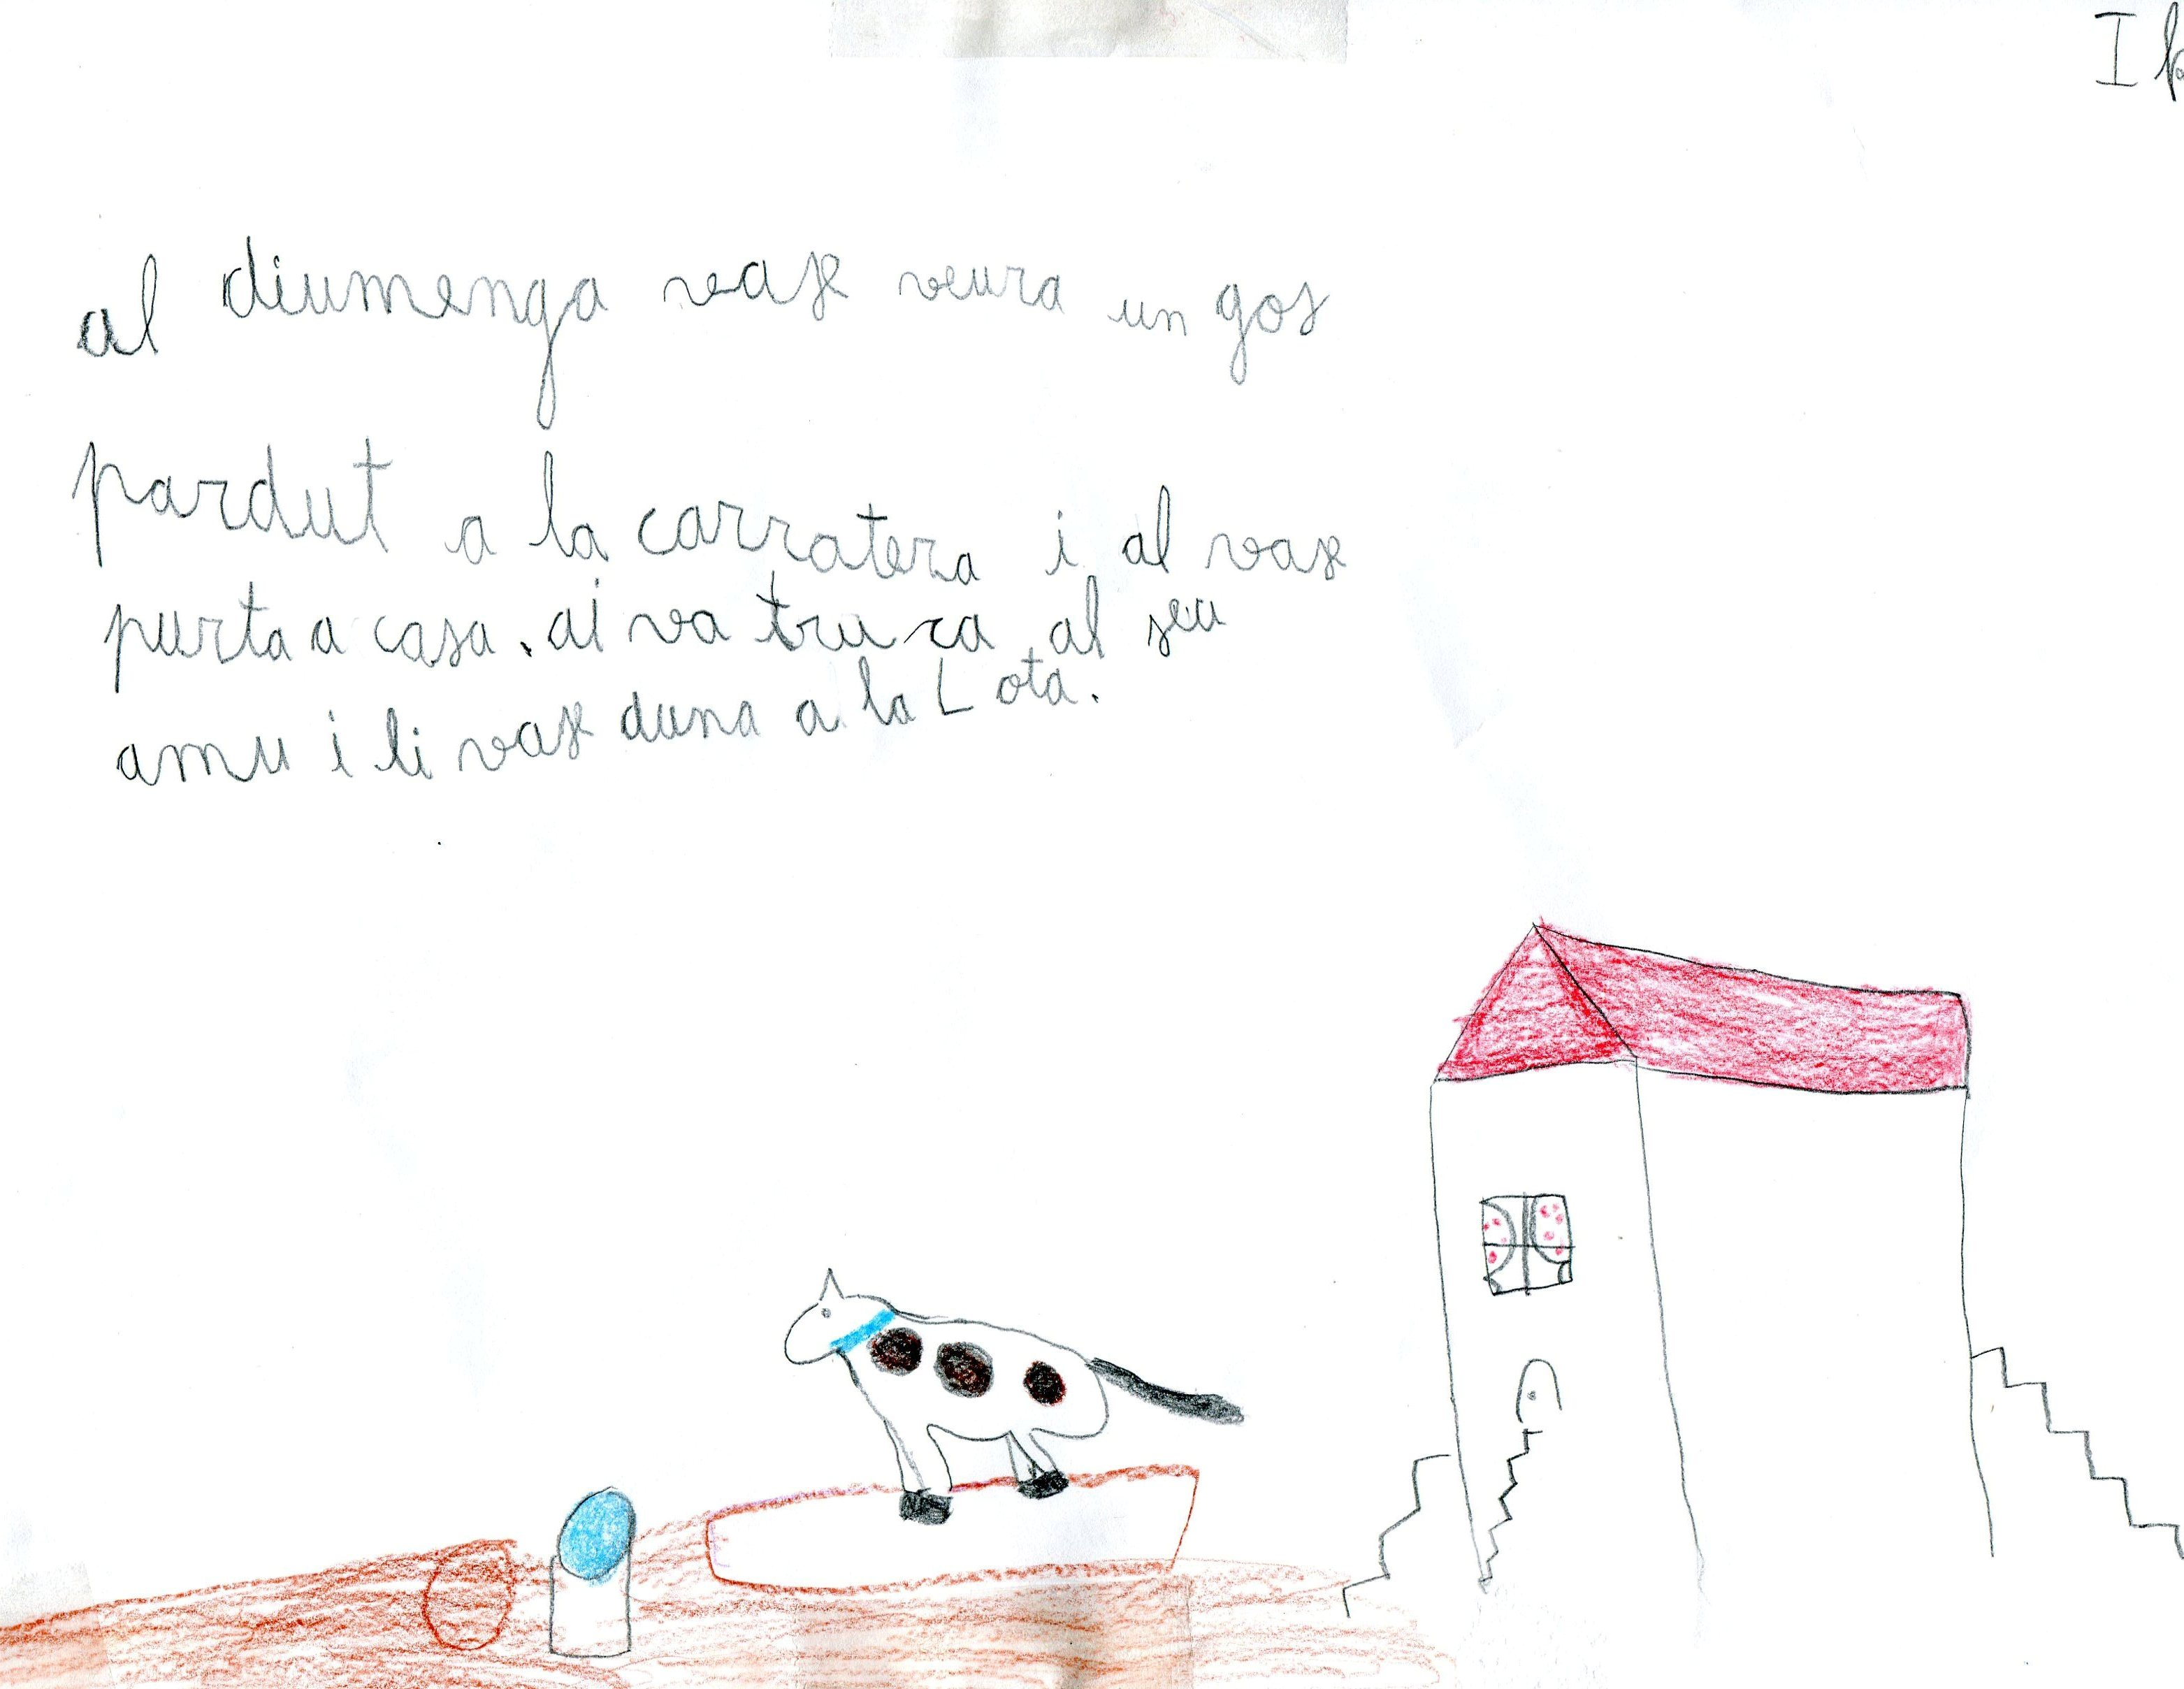
\includegraphics[width=8.4cm,keepaspectratio]{primaria/img/img010.jpg}}

\noindent\fbox{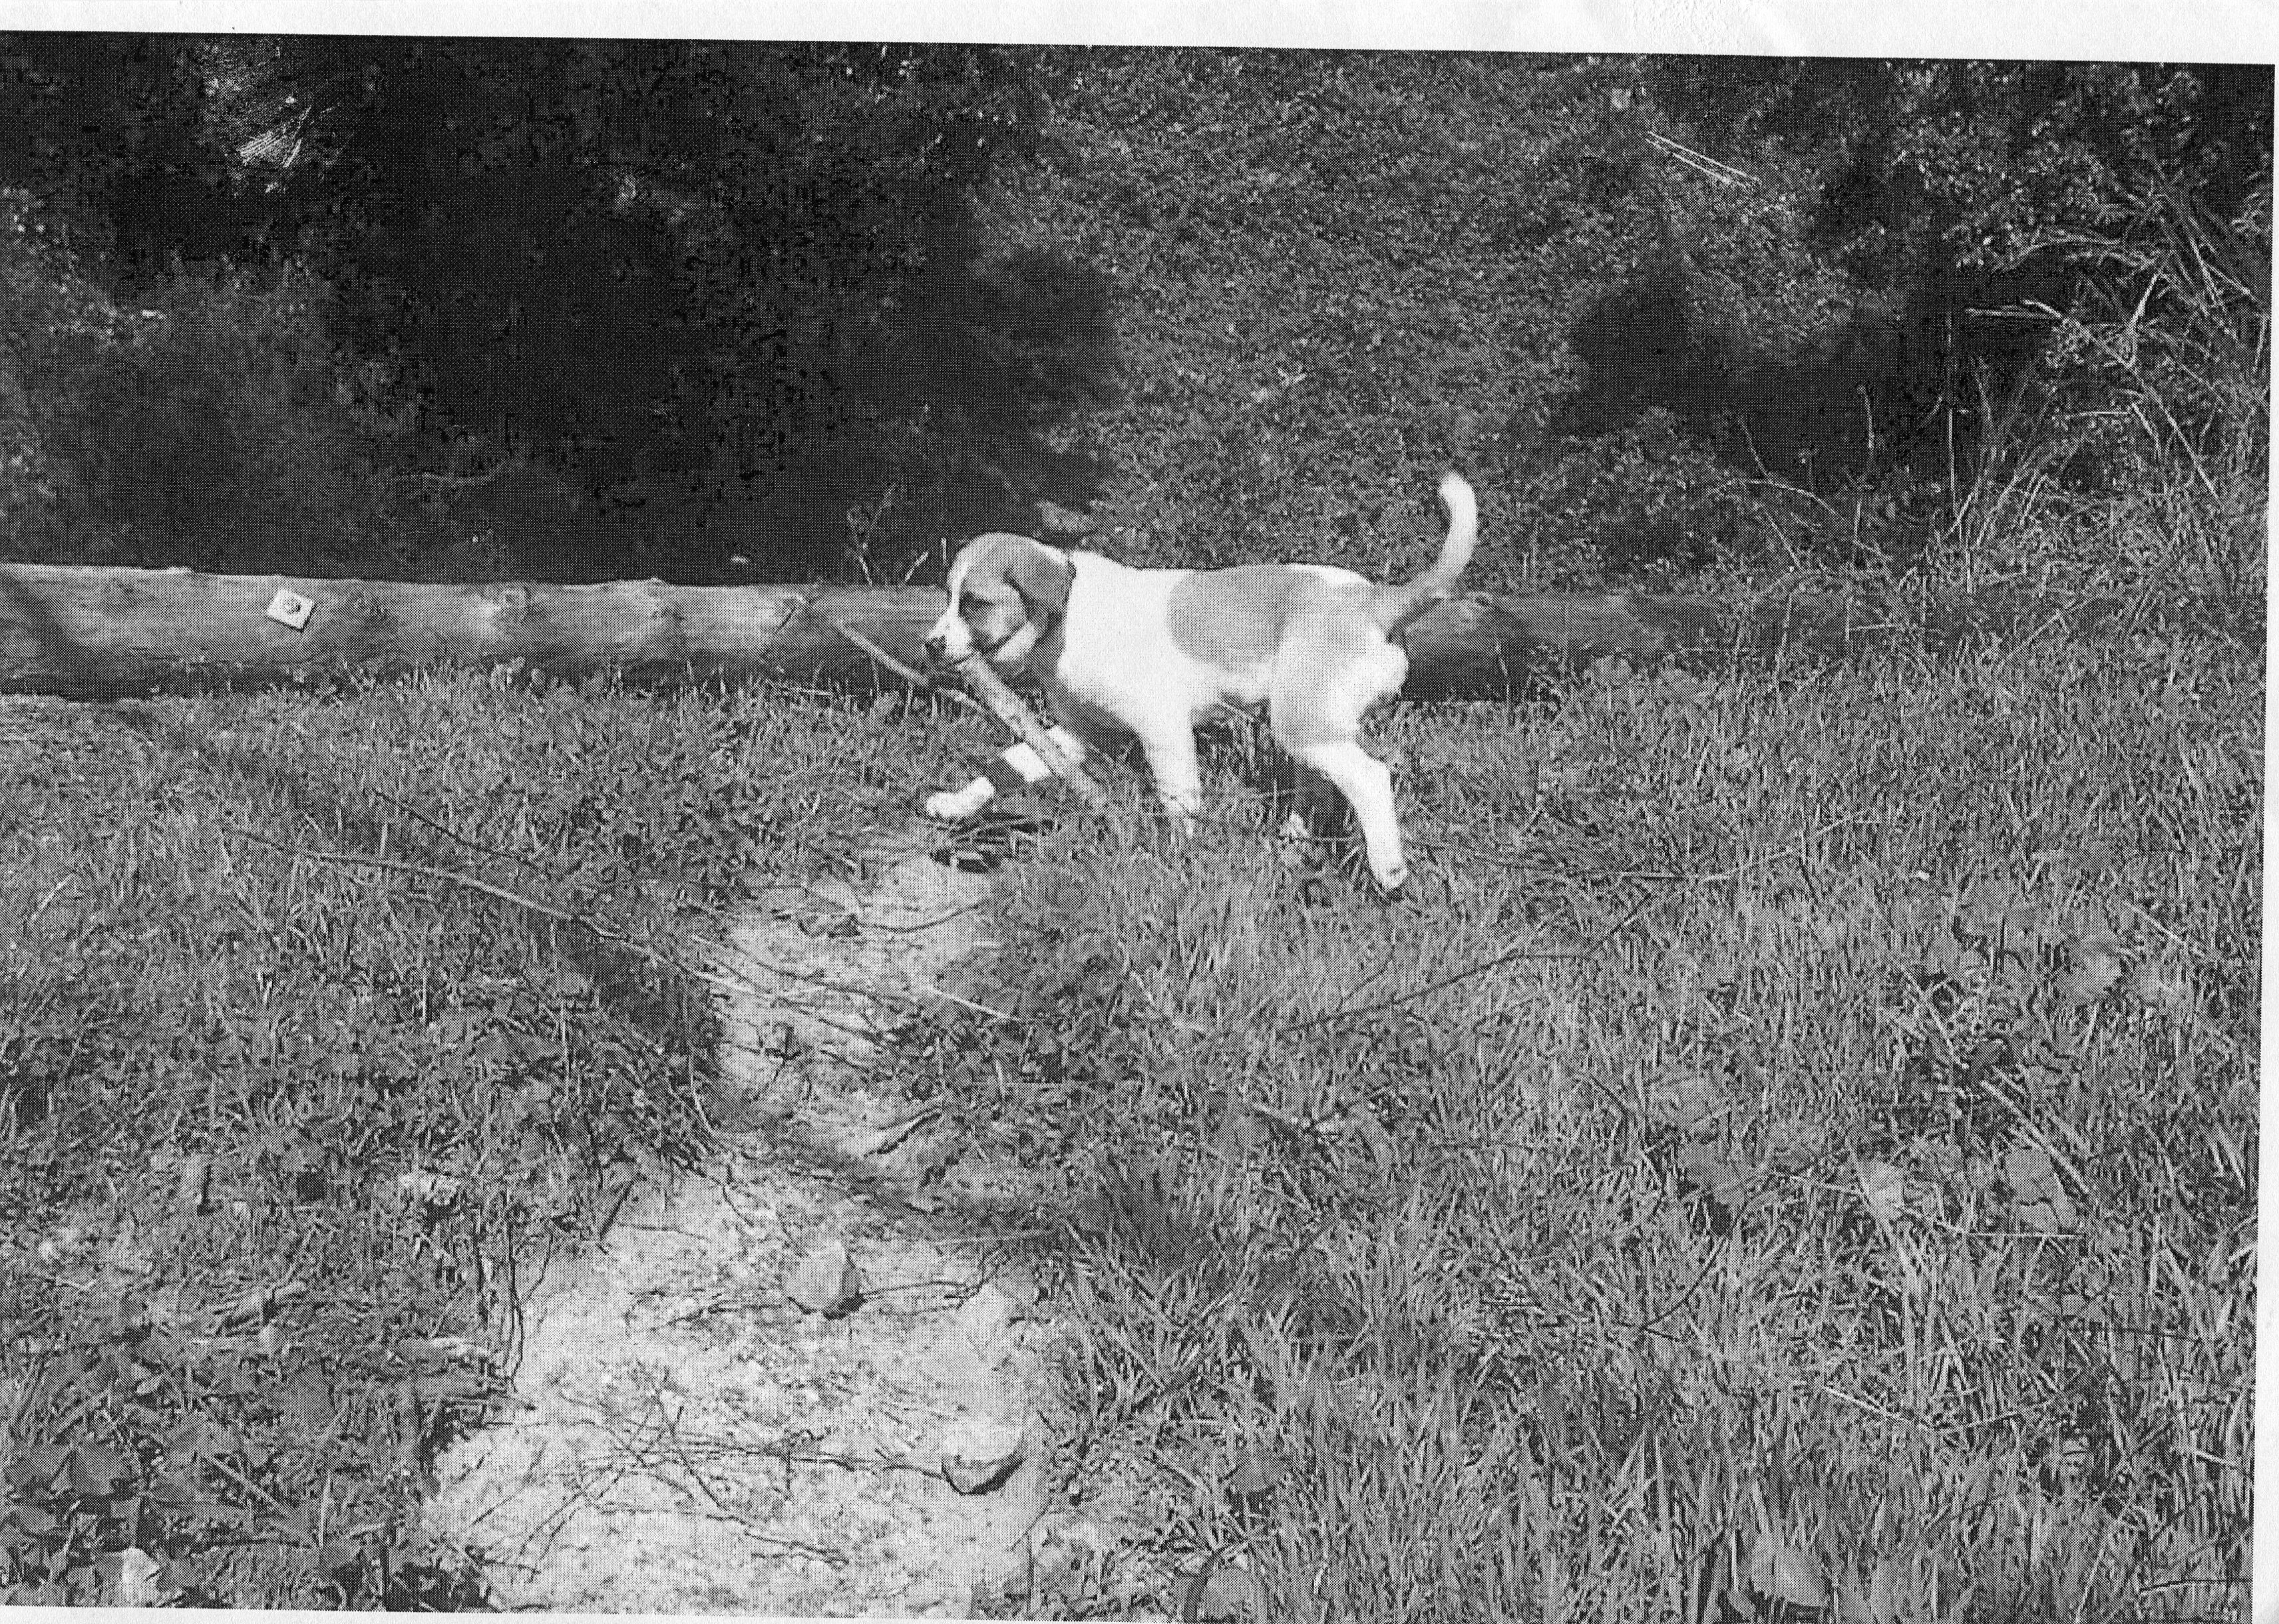
\includegraphics[width=8.4cm,keepaspectratio]{primaria/img/img011.jpg}}

\noindent\fbox{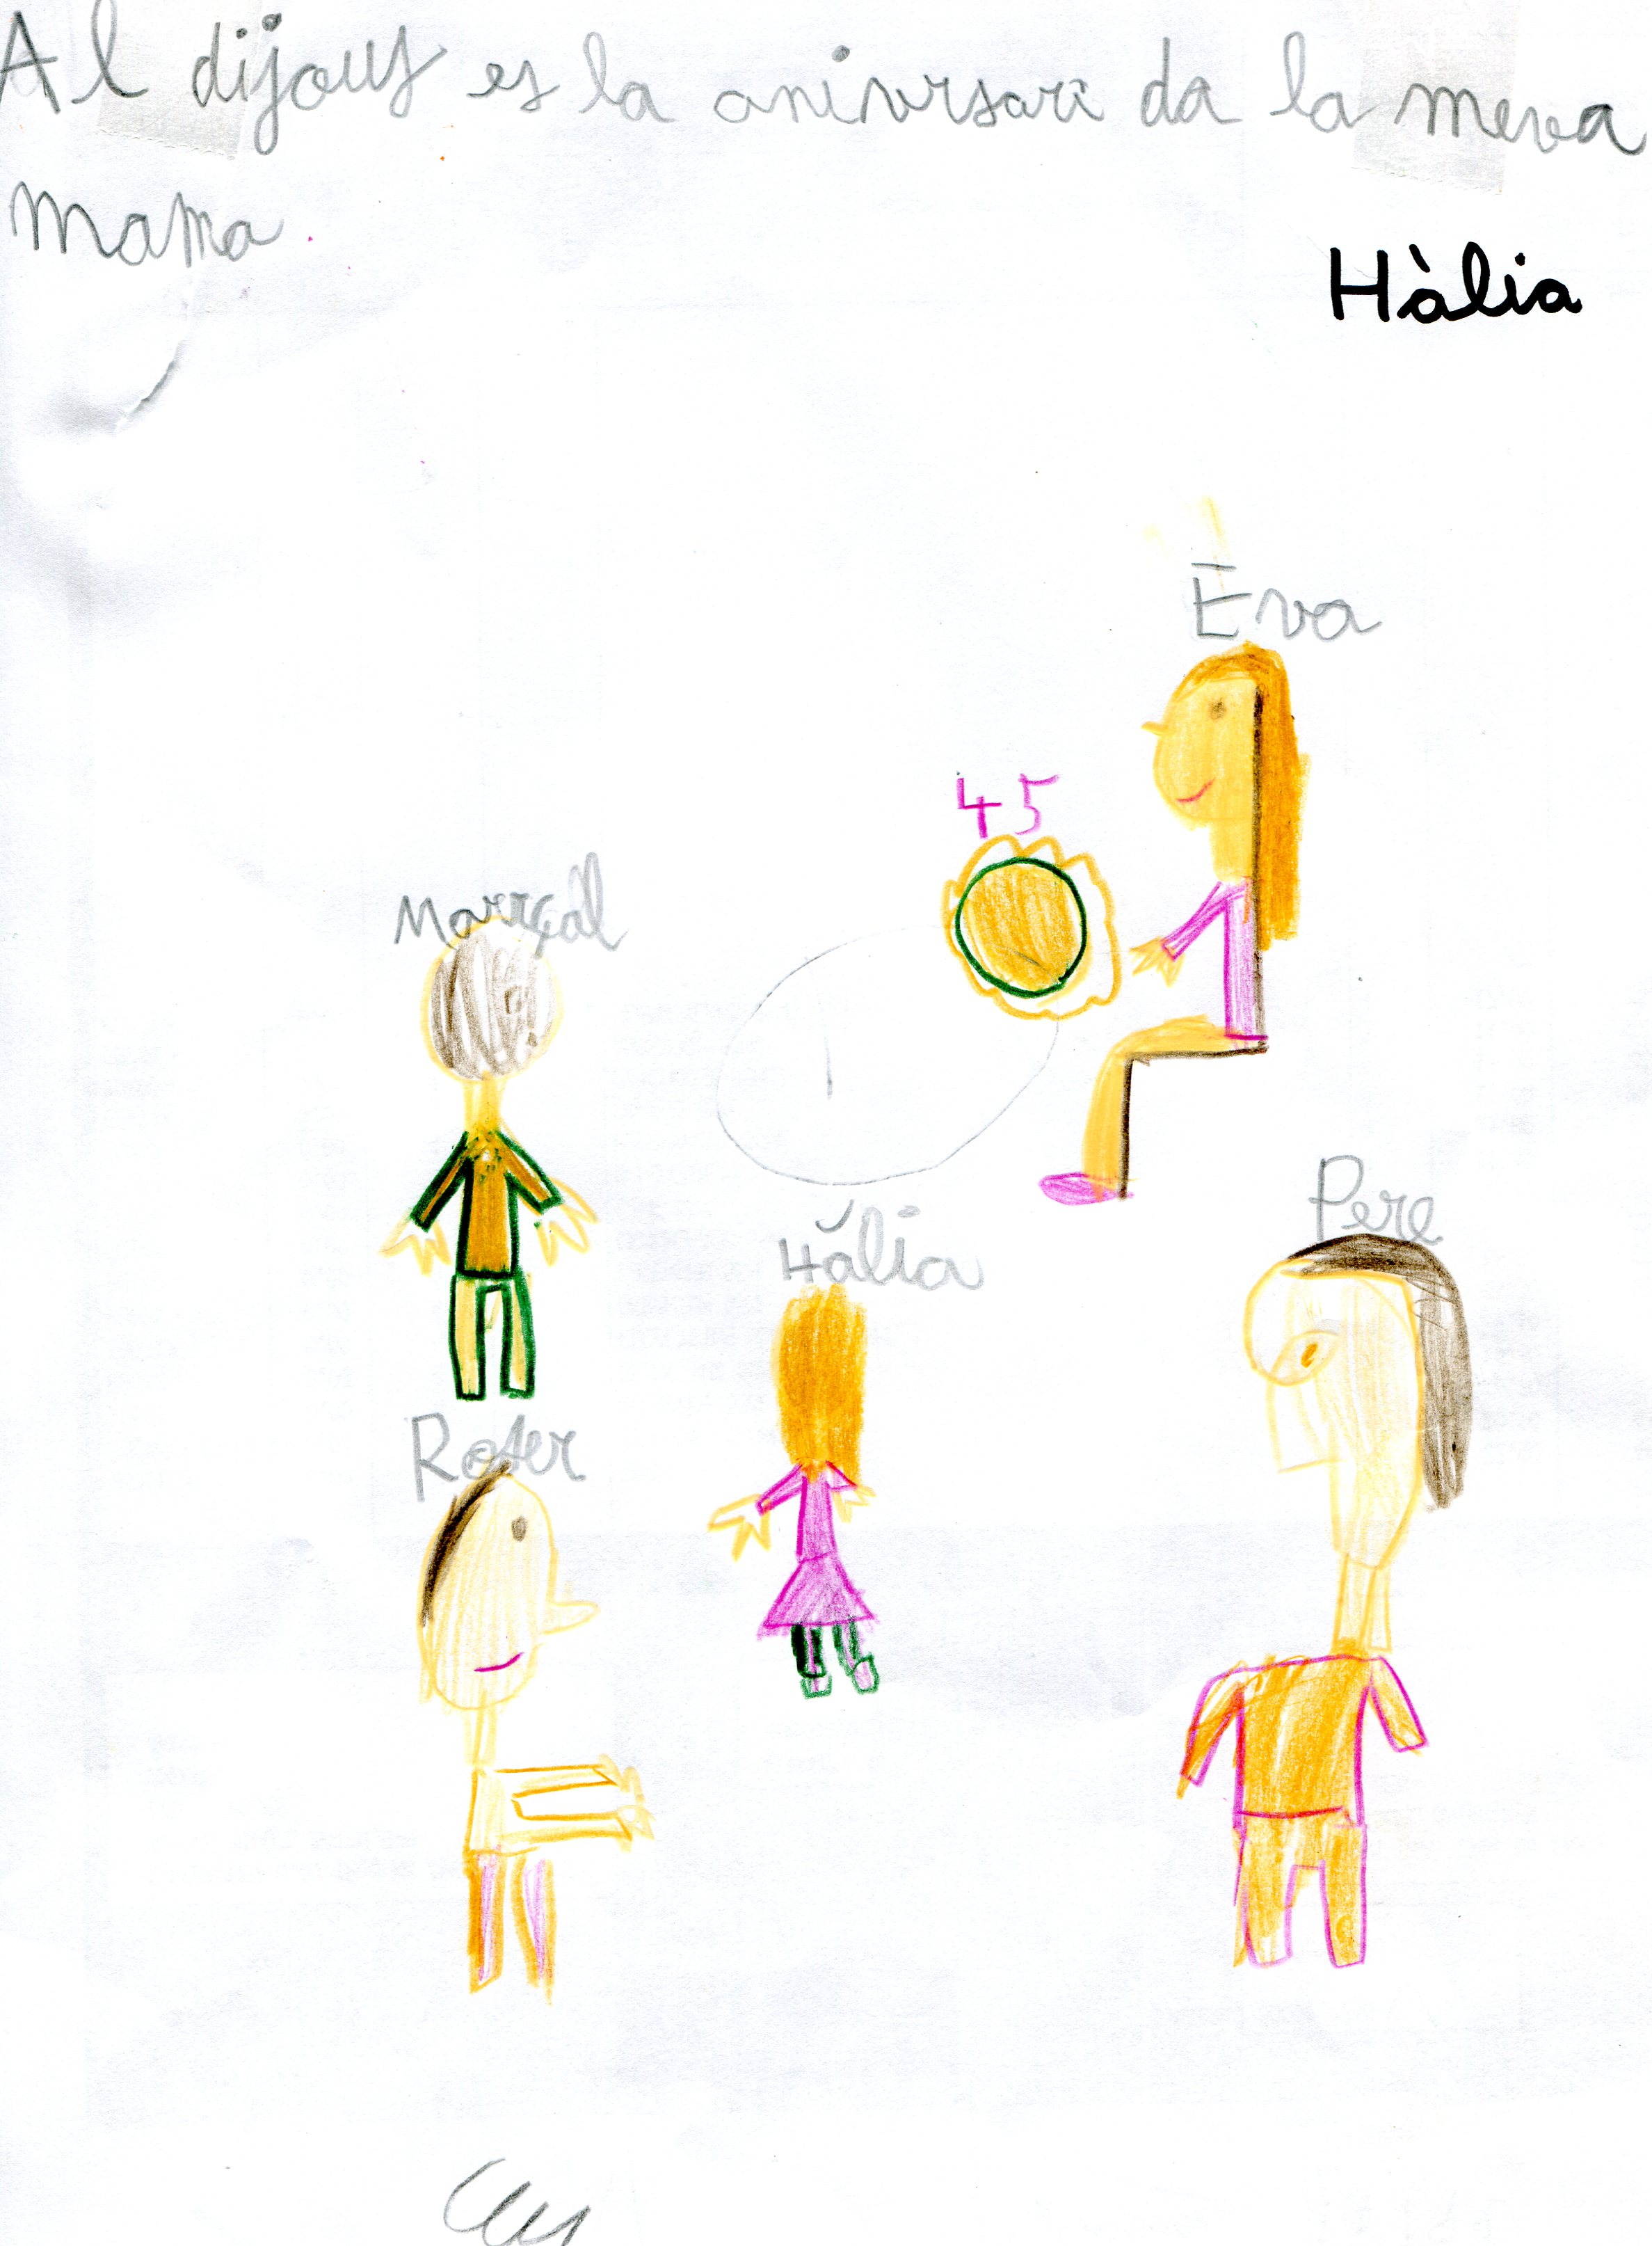
\includegraphics[width=8.4cm,keepaspectratio]{primaria/img/img012.jpg}}

\noindent\fbox{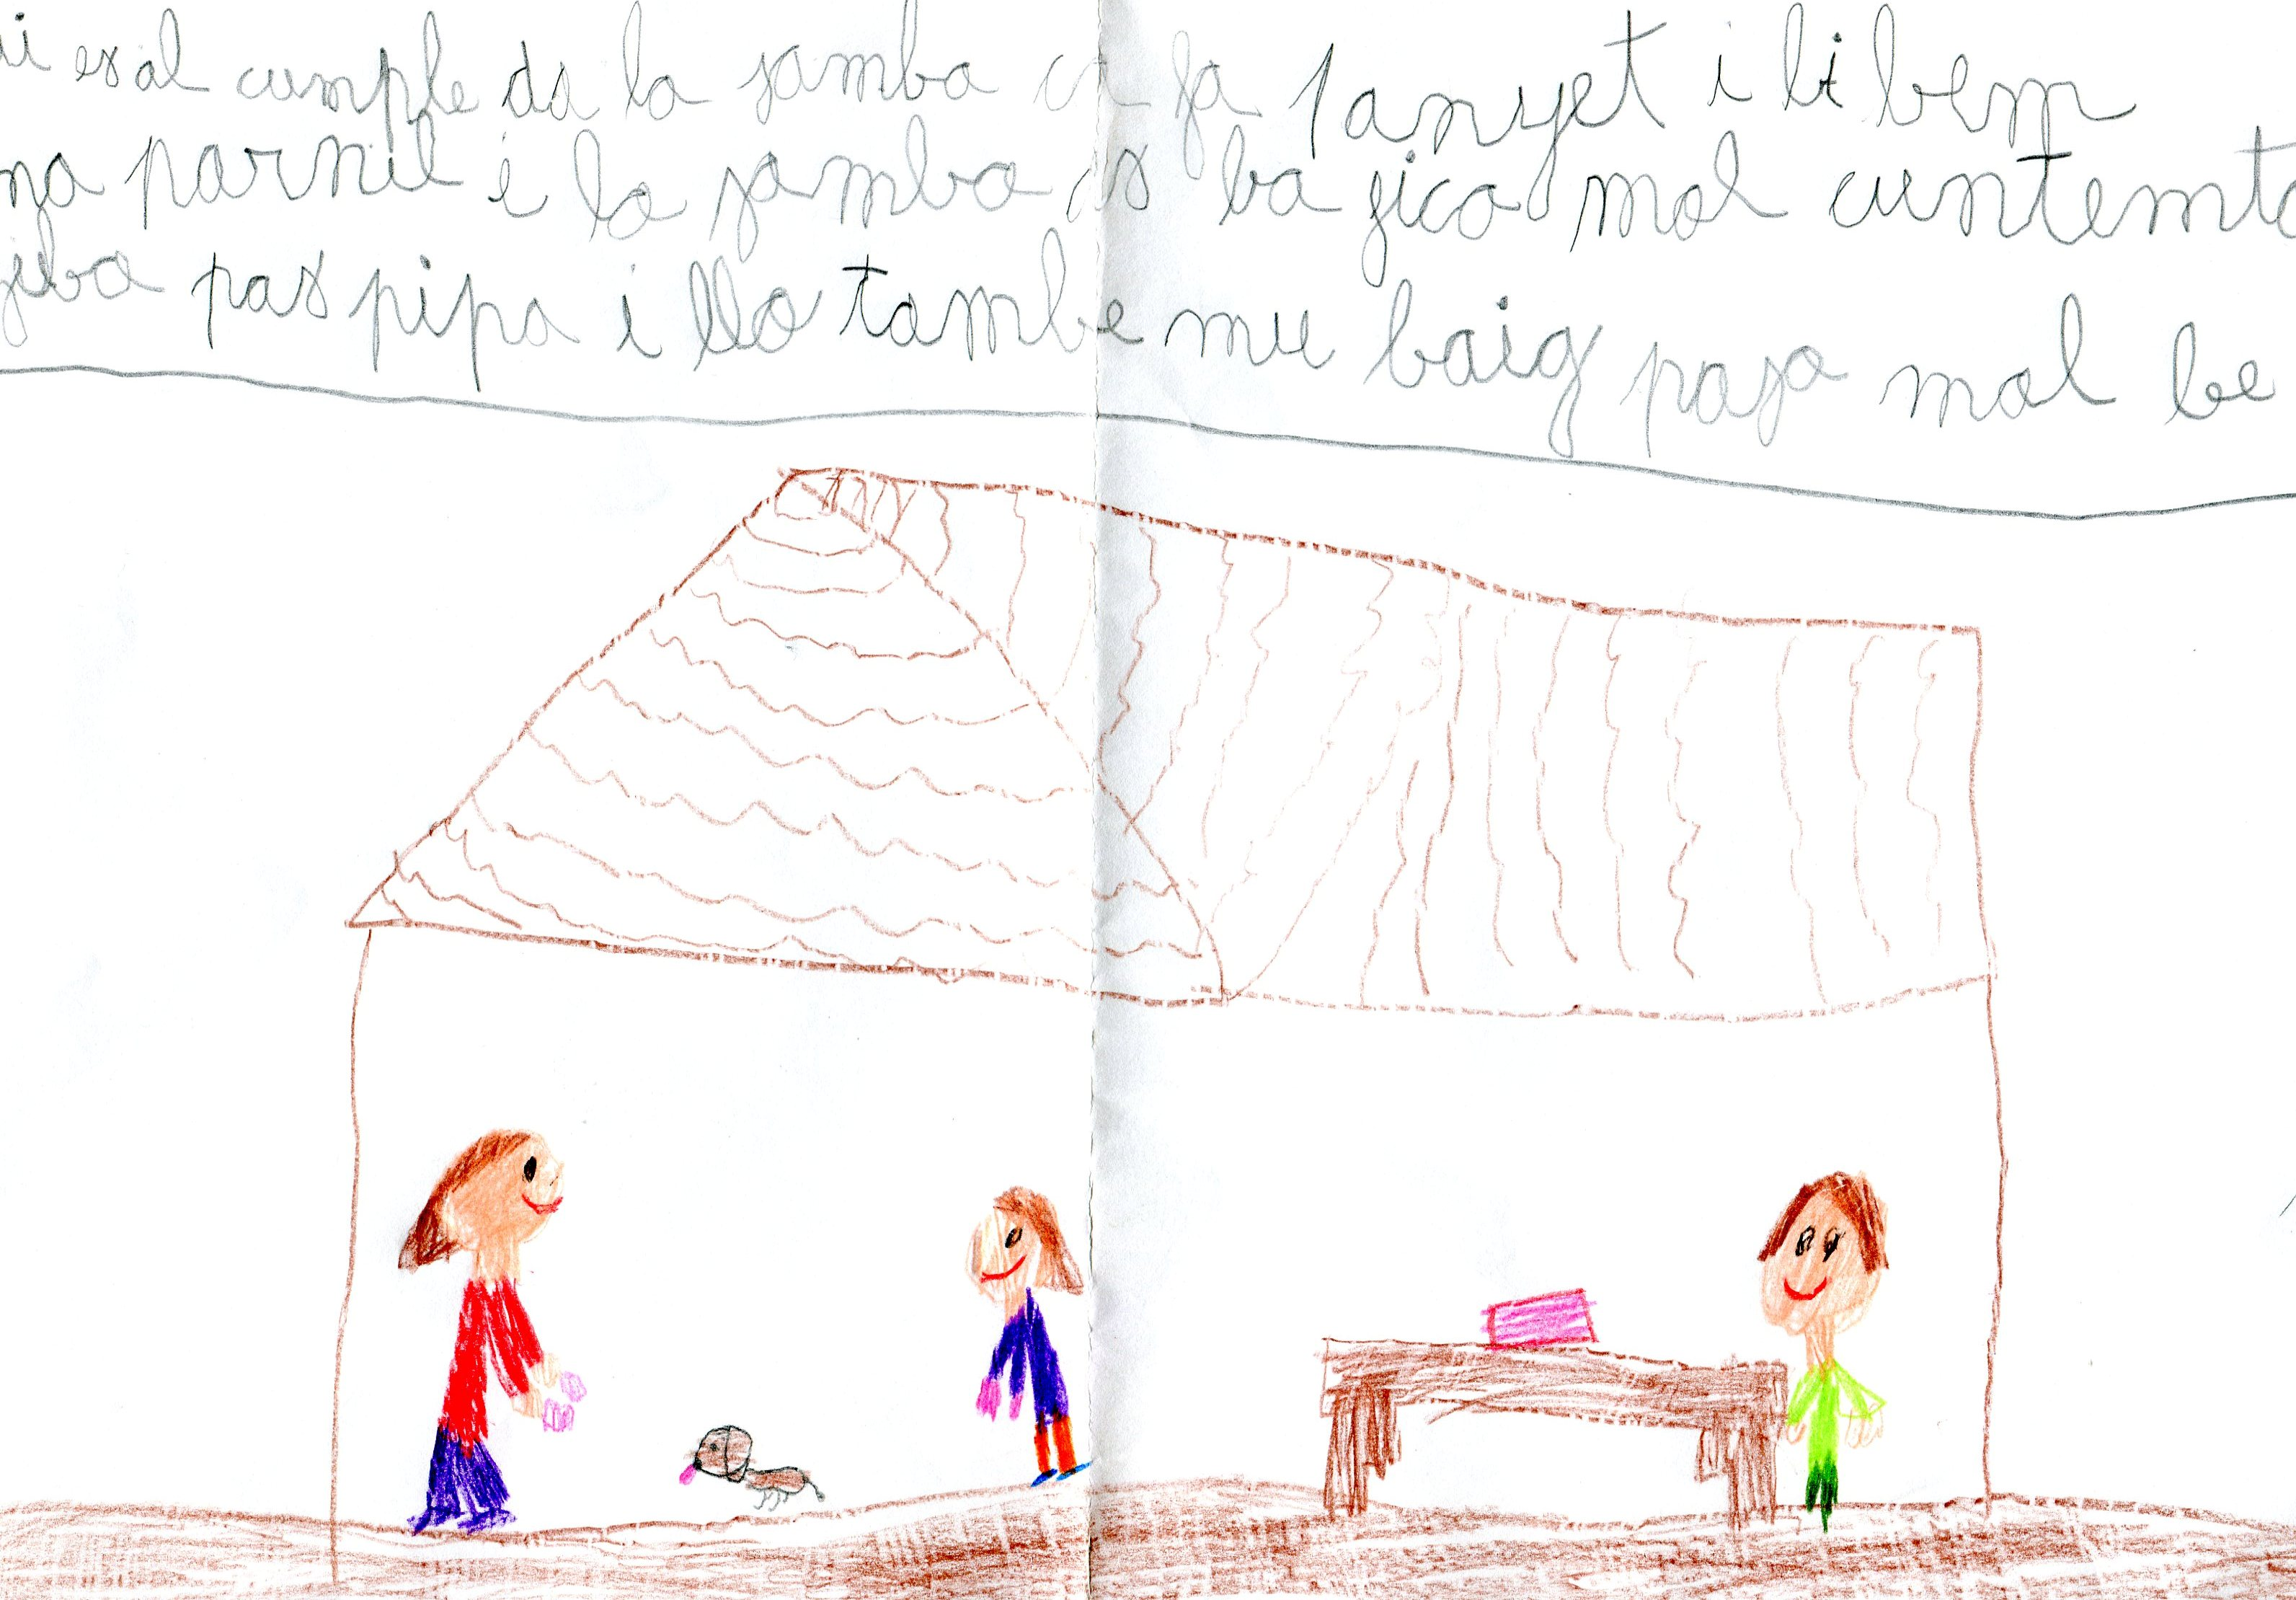
\includegraphics[width=8.4cm,keepaspectratio]{primaria/img/img013.jpg}}


\end{news}
